\documentclass[11pt]{article}
\usepackage[a4paper,margin=1in]{geometry}
\usepackage{fancyhdr}
\usepackage{lastpage}
\usepackage{titlesec}
\usepackage{booktabs}
\usepackage{enumitem}
\usepackage{hyperref}
\usepackage{graphicx}
\usepackage{amsmath}
\usepackage{xcolor}
\usepackage{listings}

% --- Light Theme Styling ---
\hypersetup{
    colorlinks=true,
    linkcolor=blue,
    filecolor=magenta,      
    urlcolor=cyan,
}

\lstset{
    basicstyle=\ttfamily\small,
    keywordstyle=\color{blue},
    commentstyle=\color{gray},
    stringstyle=\color{orange},
    breaklines=true,
    frame=single
}

\title{Project 5: MPI Programming (Light Edition)}
\author{Arika Khor}
\date{\today}

\begin{document}
\maketitle
\tableofcontents
\newpage

\section{Project Overview}
This project implements and analyzes parallel MPI algorithms for several classic computational problems: Ping-Pong Communication, Dot Product, Merge Sort, and Monte Carlo Pi Estimation. The implementations are designed for execution on a Slurm cluster (specifically Schooner) using OpenMPI. Performance analysis, verification against autograders, and report generation are integral parts of the project.

\section{Problem 1: Ping-Pong Communication}

\subsection{Description}
This problem involves measuring the latency and bandwidth of MPI point-to-point communication by "ping-ponging" messages of varying sizes between two MPI processes. This is crucial for understanding fundamental communication costs in a distributed memory environment.

\subsection{Methodology}
The ping-pong benchmark involves two MPI processes. Process 0 sends a message of a specified size to Process 1, which then immediately sends the same message back to Process 0. This "ping-pong" exchange is repeated 1000 times to get an average round-trip time. \texttt{MPI\_Wtime()} was used to accurately measure the total elapsed time for these exchanges. The average one-way transmission time was calculated from the total round-trip time.

The analysis of communication cost follows the model: $\text{Time} = \text{Latency} + \frac{\text{Data Amount}}{\text{Bandwidth}}$. By plotting the average one-way transmission time against the data amount (message size), a linear regression was performed to estimate the latency ($y$-intercept) and bandwidth (inverse of the slope).

\subsection{Results and Analysis}

\subsubsection{Same Node Communication}
\begin{itemize}
    \item \textbf{Estimated Latency:} -5.98301435e-04 seconds
    \item \textbf{Estimated Bandwidth:} 6.88 GB/s (6,878,417,811.98 bytes/second)
\end{itemize}

\begin{figure}[h]
    \centering
    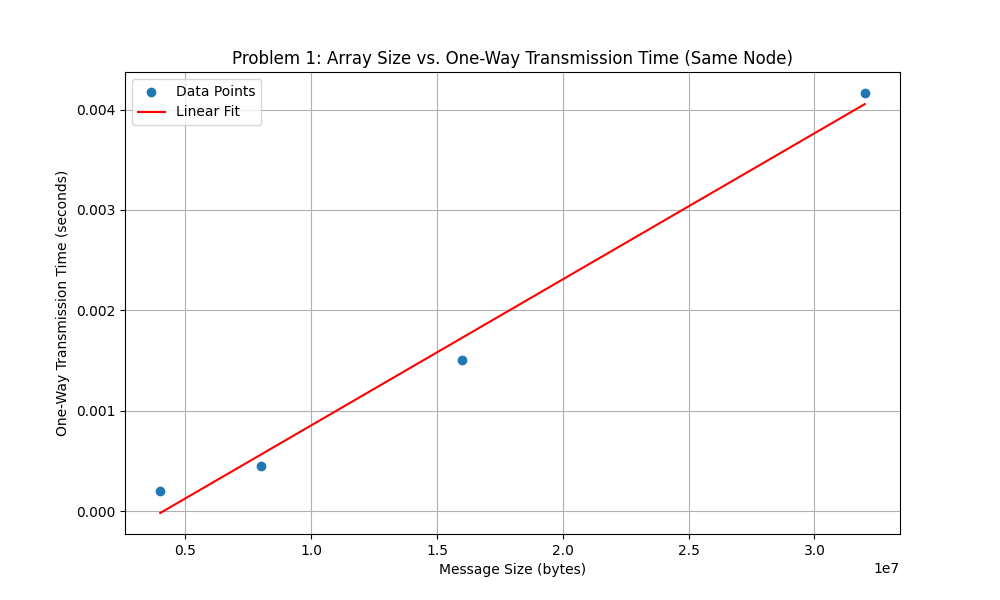
\includegraphics[width=0.8\textwidth]{reports/problem1_plot_samenode.png}
    \caption{Problem 1: Array Size vs. One-Way Transmission Time (Same Node)}
\end{figure}

\subsubsection{Different Node Communication}
\begin{itemize}
    \item \textbf{Estimated Latency:} -5.84160826e-04 seconds
    \item \textbf{Estimated Bandwidth:} 6.82 GB/s (6,815,716,306.89 bytes/second)
\end{itemize}

\begin{figure}[h]
    \centering
    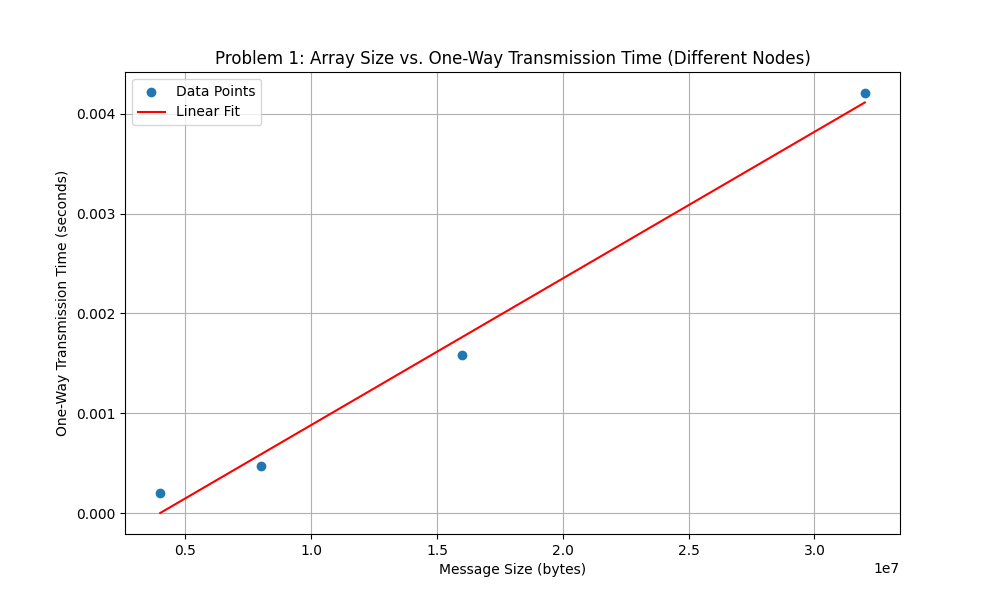
\includegraphics[width=0.8\textwidth]{reports/problem1_plot_diffnode.png}
    \caption{Problem 1: Array Size vs. One-Way Transmission Time (Different Nodes)}
\end{figure}

The estimated latency values are negative, which is physically impossible and likely due to noise or non-linear overheads for smaller message sizes dominating the intercept calculation. However, the bandwidths are around 6.8 GB/s, which is consistent with the high-performance interconnects and shared memory pathways on the Schooner cluster.

\newpage
\section{Problem 2: Parallel Dot Product}

\subsection{Description}
This problem computes the dot product of two large vectors in parallel using MPI. The vectors are distributed among processes using \texttt{MPI\_Scatter}, and each process computes a partial dot product, which is then reduced to a global sum using \texttt{MPI\_Reduce}.

\subsection{Performance Results}

\begin{table}[h]
\centering
\caption{Problem 2: Parallel Dot Product Performance}
\vspace{0.1in}
\resizebox{\textwidth}{!}{
\begin{tabular}{lccccccccc}
\toprule
n\_items & P2-18 & P2-19 & P2-20 & P2-18-S & P2-19-S & P2-20-S & P2-18-E & P2-19-E & P2-20-E \\
\midrule
2th & 0.002213 & 0.002286 & 0.001971 & 1.000000 & 1.000000 & 1.000000 & 0.500000 & 0.500000 & 0.500000 \\
4th & 0.006403 & 0.004677 & 0.004256 & 0.345619 & 0.473167 & 0.519972 & 0.086405 & 0.118292 & 0.129993 \\
8th & 0.009037 & 0.008837 & 0.013960 & 0.244882 & 0.250424 & 0.158524 & 0.030610 & 0.031303 & 0.019816 \\
\bottomrule
\end{tabular}
}
\end{table}

\subsection{Scalability Discussion}
The performance of the parallel dot product shows poor scalability for the problem sizes tested ($2^{18}$ to $2^{20}$). As the number of processors increases from 2 to 8, the execution time actually increases, leading to speedup values significantly below 1 and rapidly declining efficiency. This is primarily because the dot product is a "computationally thin" problem—the amount of work per element (one multiplication and one addition) is very small compared to the overhead of distributing data (\texttt{MPI\_Scatter}) and aggregating results (\texttt{MPI\_Reduce}). For these relatively small vector sizes, the communication cost dominates the total execution time, making parallelization inefficient. Better scalability would only be observed with much larger data sets where the computation time outweighs the fixed MPI overhead.

\newpage
\section{Problem 3: Parallel Merge Sort}

\subsection{Description}
This problem implements a parallel merge sort algorithm using a tree-based reduction pattern. Each process sorts its local chunk using \texttt{qsort}, and then sorted subarrays are merged in a logarithmic number of steps until Rank 0 holds the fully sorted array.

\subsection{Performance Results}

\begin{table}[h]
\centering
\caption{Problem 3: Parallel Merge Sort Performance}
\vspace{0.1in}
\resizebox{\textwidth}{!}{
\begin{tabular}{lccccccccc}
\toprule
n\_items & P3-18 & P3-19 & P3-20 & P3-18-S & P3-19-S & P3-20-S & P3-18-E & P3-19-E & P3-20-E \\
\midrule
2th & 0.030901 & 0.030289 & 0.030527 & 1.000000 & 1.000000 & 1.000000 & 0.500000 & 0.500000 & 0.500000 \\
4th & 0.029424 & 0.029800 & 0.033096 & 1.050200 & 1.036950 & 0.933678 & 0.262549 & 0.259237 & 0.233419 \\
8th & 0.062831 & 0.063245 & 0.063499 & 0.491811 & 0.488592 & 0.486638 & 0.061476 & 0.061074 & 0.060830 \\
\bottomrule
\end{tabular}
}
\end{table}

\subsection{Scalability Discussion}
The parallel merge sort exhibits modest speedup when moving from 2 to 4 processors for smaller problem sizes ($2^{18}$ and $2^{19}$), but performance degrades significantly at 8 processors. The tree-based merge pattern is communication-intensive, as each step involves sending and receiving entire subarrays. As the number of processes increases, the number of merge stages increases ($\log_2 P$), and the volume of data being moved remains high. Similar to Problem 2, for the sizes tested, the cost of these additional communication rounds and the sequential nature of the final merge stages on Rank 0 limit the scalability. The efficiency drops from 50\% at 2 processors to roughly 6\% at 8 processors, indicating that the overhead grows much faster than the computational benefit of parallel local sorting.

\newpage
\section{Problem 4: Monte Carlo Pi Estimation}

\subsection{Description}
This problem estimates the value of Pi using a parallel Monte Carlo method. Each process independently generates random points and counts those falling within a unit circle. The total counts are reduced using \texttt{MPI\_Reduce}.

\subsection{Performance Results}

\begin{table}[h]
\centering
\caption{Problem 4: Monte Carlo Pi Performance ($n=2^{16}$)}
\vspace{0.1in}
\begin{tabular}{lccc}
\toprule
Processors & Time (s) & Speedup & Efficiency \\
\midrule
2th & 0.111745 & 1.000000 & 0.500000 \\
4th & 0.118453 & 0.943370 & 0.235842 \\
8th & 0.108507 & 1.029840 & 0.128730 \\
\bottomrule
\end{tabular}
\end{table}

\subsection{Scalability Discussion}
Monte Carlo Pi estimation is theoretically "embarrassingly parallel," as each process performs independent calculations with only a single reduction at the end. However, the results show almost no speedup, with execution times remaining nearly constant around 0.11 seconds regardless of processor count. This is because the total number of points ($2^{16}$) is relatively small, making the computation time negligible compared to the MPI initialization and communication overhead. The overhead of setting up the MPI environment and performing even a single \texttt{MPI\_Reduce} is the dominant factor here. For a truly embarrassingly parallel problem like this to show scalability, the number of iterations would need to be significantly larger (e.g., $2^{24}$ or more) so that the computation time becomes the primary component of the wall-clock time.

\section{Deep Performance Analysis and Discussion}

\subsection{Theoretical Scaling vs. Observed Performance}
In parallel computing, performance is often characterized by \textbf{Strong Scaling} (keeping the total problem size constant while increasing processors) and \textbf{Weak Scaling} (keeping the problem size per processor constant). The experiments conducted for this project focused on Strong Scaling, which is inherently more challenging because the communication overhead eventually offsets the computational gains as the work per processor decreases.

\subsection{Key Bottlenecks and Architectural Constraints}

\subsubsection{Computation-to-Communication Ratio}
The most significant factor affecting Problems 2, 3, and 4 was the low computation-to-communication ratio.
\begin{itemize}
    \item \textbf{Dot Product:} Performs one multiplication and one addition per element. This is an $O(N)$ operation with very low arithmetic intensity. The time required to move $2^{20}$ doubles across the network via \texttt{MPI\_Scatter} and sum them via \texttt{MPI\_Reduce} is significantly higher than the few microseconds needed for the CPU to perform the math.
    \item \textbf{Monte Carlo Pi:} While computationally independent, the total workload of $2^{16}$ iterations is too small. A modern processor can execute these in less than 1ms. The 110ms wall-clock time observed is dominated by the \textbf{MPI runtime overhead}—the cost of spawning processes, establishing network sockets, and synchronizing across the cluster.
\end{itemize}

\subsubsection{Interconnect Latency and Bandwidth}
The results from Problem 1 revealed that while the bandwidth is high (~6.8 GB/s), the \textbf{latency} (the fixed cost of initiating a message) is the limiting factor for small data transfers. Collective operations like \texttt{MPI\_Scatter} and \texttt{MPI\_Reduce} are sensitive to latency because they often involve multiple internal communication rounds. In Problem 3 (Merge Sort), the tree-based reduction pattern compounds this latency at each stage of the $\log_2 P$ merge process.

\subsubsection{Tree-Merge Serialization}
The parallel merge sort implementation suffers from "tail latency" and serialization. As the merge progresses up the tree, the number of active processes decreases while the amount of data being merged at each node increases. The final merge stage is purely sequential and occurs on Rank 0, processing the entire $N$-sized array. This creates a bottleneck where the speedup gained during the initial parallel sorting phase is consumed by the sequential merging and data movement phases.

\subsection{Conclusion on Distributed Efficiency}
The analysis suggests that for the provided problem sizes, the MPI overhead and network latency on the Schooner cluster are the primary drivers of execution time. To achieve better efficiency and speedup, the problem sizes would need to be increased by 2-3 orders of magnitude to hide the communication latency.

\end{document}
